\documentclass[en,hazy,blue,screen,14pt]{elegantnote}
\usepackage[T1]{fontenc}
\usepackage[latin9]{inputenc}
\usepackage{babel}
\usepackage{float}
\usepackage{textcomp}
\usepackage{amsmath,amsfonts,amssymb}
\usepackage{amsthm}
\usepackage{graphicx}
\usepackage[ruled,vlined]{algorithm2e}
\PassOptionsToPackage{normalem}{ulem}
\usepackage{ulem}
\usepackage{mathtools}
\DeclarePairedDelimiter{\ceil}{\lceil}{\rceil}

\title{Class Notes\\CIS 502 Analysis of Algorihtm\\3-Graph Traversal}
\author{Da Kuang}
\institute{University of Pennsylvania}
% \version{1.00}
\date{}

\begin{document}

\maketitle
\newpage
\section{Graphics Basics}
\begin{itemize}
\item A graph G is an ordered pair of two sets $(V, E)$.
\item $V$ is a set of vertices/points/nodes, which is always a finite set.
\item $E$ is a set of unordered pair of vertices.
\item An edge is represented as $(u ,v)$. Here we abuse the notion of ordered 
pair to represent unordered pair.
\end{itemize}
% \centerline{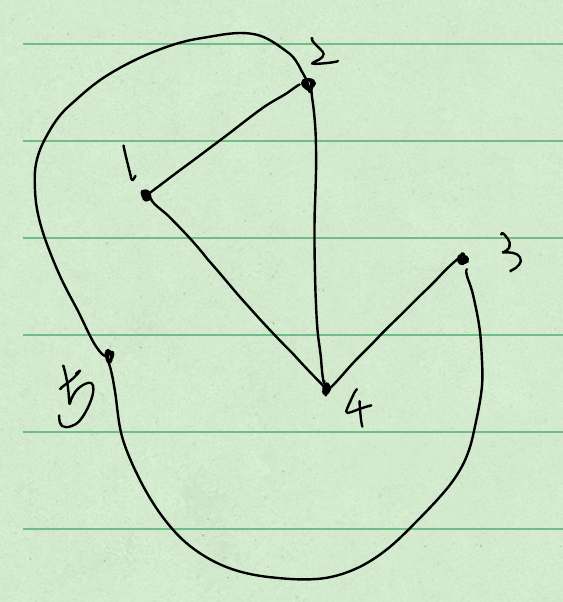
\includegraphics[width=0.2\textwidth]{graph.png}}

\subsection{Two representation of Graph}
When we talked about graph without adjective, that mean it is a 
undirected graph. Suppose the number of vertices is $|V| = n$.
\begin{itemize}
 \item A vertex is incident to an edge if the vertex is one of the two vertices 
the edge connects.
\item If an edge $(u, v)$ has end points $u$ and $v$, we say it is an incident 
to vertex $u$ and $v$.
\item $u$, $v$ are adjacent if $(u, v) \in \mathbb{E}$.
\item The degree of vertex $v$ is the number of edges incident on $v$.
\end{itemize}

\subsubsection{Adjacency Matrix}
Adjacency Matrix is an sysmetric matrix for undirected graph where
\[
V_{ij} = 
\begin{cases*}
 |(i,j)| & ,\text{ if $(i,j) \in \mathbb{E}$.}\\
 0  &,\text{ otherwise.}
\end{cases*}
\]
\subsubsection{Adjacency List}
Adjacency List is an array of size n of linked list, where $i$-th entry is 
a linked list consisting of the neighbos of vertex-$i$. It is default 
representation of graph.

Space = $O(n + m)$
\subsection{Connectivity}
\subsubsection{Path}
A path in a graph is a sequence of vertices
\[v_0 v_1 \cdots v_k\]
, such that $(v_i, v_{i+1}) \in \mathbb{E}$ for $i = 0, 1, 2, \cdots, k-1$
A simple path is a path that does not repeat vertices.
\paragraph{Lemma:}
If there is a path $(u, v)$, there must be a simple path $(u, v)$.
\subsubsection{Cycle}
A cycle in a graph is a sequence of vertices
\[v_0 v_1 \cdots v_kv_0\]
, such that $(v_i, v_{i+1}) \in \mathbb{E}$ for $i = 0, 1, 2, \cdots, k-1$ and 
$(v_k, v_{0}) \in \mathbb{E}$. All $v_i$s are distinct.

\subsubsection{Connectivity}
\begin{itemize}
 \item $u$, $v$ is \textbf{connected} if there is a path between them.
 \item $G$ is \textbf{connected} if $\forall u, v \in V$, there is a path 
between $u$ and $v$.
\item The \textbf{connected components} of $G$ are maximal subset of vertices 
that are pairwise connected.
\end{itemize}

\subsubsection{Connection is equivalence relation}
Connection relation in a graph is an equivalence relation.
\begin{itemize}
 \item Reflexive Relation (take Path of length 0)
 \item Symmetric Relation (reversible path)
 \item Transitive Relation: If a Graph has a $uv$ path and also $vw$ path then 
it will also contain $uw$ path.
\end{itemize}
Because connnection is the equivalence relation, pairwise connected vertices 
form a connected component.
\section{Tree}
Tree is a connected acyclic graph.
\subsection{Rooted tree}
\subsubsection{Inductive Defintion}
A nice thing about Inductive defintion is it is useful for the proofs by 
induction.
\begin{itemize}
 \item \textbf{Rule 1:} A graph consist of a single vertex v is a rooted tree 
with v as the root.
 \item \textbf{Rule 2:} If $(T_1, r_1)$, $(T_2, r_2), \cdot, (T_k, r_k)$ are 
rooted trees, then the tree $(T, r)$ consisting of a new node $r$ as root and 
edges $(r, r_1), \cdots, (r, r_k)$ is a rooted tree.
\end{itemize}
\subsection{Structural induction Proof}
Statement: Any tree with $n$ nodes has $n-1$ edges.

Since any tree can be transformed into a rooted tree, the induction can be as 
following:
\begin{itemize}
 \item Statement: Any rooted tree on $n$ nodes has $n-1$ edges.
 \item Base case: Single node tree with no edge. The statement is true.
 \item Inductive hypothesis: For a rooted tree $T_r$, built up from $(T_1, 
r_1), (T_2, r_2), \cdots, (T_n, r_n)$ using rule 2. Assume the statement is 
true for all the trees $T_1, T_2, \cdots, T_k$ and prove it for $t$.
\item Inductive step:
    \begin{itemize}
    \item Let tree $T_i$ have $n_i$ nodes, $i = 1, 2, \cdots, k$. Then $T$ has 
    $\sum_{i=1}^k n_i + 1$ nodes.
    \item By the inductive hypothesis, $T_i$ has $n_i - 1$ edges.
    \item Total number of edges is $T = \sum_{i=1}^k (n_i - 1) + k = 
\sum_{i=1}^k 
    n_i$.
    \item The number of edge is one less than the number of nodes. It proofs 
the     inductive step.
    \end{itemize}
 \end{itemize}
\section{Traversal}
Traversal: Visiting all parts of the graph.
\subsection{Traversal rooted tree}
\subsubsection{Post-order traversal}
\begin{itemize}
\item First traverse each of the children 
\item Visit the root.
\end{itemize}






\end{document}
